\documentclass[tikz,border=3mm]{standalone}

\usepackage{amsmath,amssymb}
\usepackage{xcolor}
\usepackage{helvet}
\renewcommand{\familydefault}{\sfdefault}
\usetikzlibrary{arrows.meta,positioning,fit,calc,backgrounds}

\definecolor{ink}{HTML}{111827}
\definecolor{muted}{HTML}{4B5563}
\definecolor{prebg}{HTML}{DFF1FB}
\definecolor{frontbg}{HTML}{F1E4FA}
\definecolor{backbg}{HTML}{E7F5EA}
\definecolor{blue}{HTML}{0EA5E9}
\definecolor{green}{HTML}{16A34A}
\definecolor{red}{HTML}{DC2626}
\definecolor{violet}{HTML}{7C3AED}
\definecolor{amber}{HTML}{D97706}
\definecolor{darkbox}{HTML}{374151}

\tikzset{
  >=Latex,
  sectiontitle/.style={font=\bfseries\large, text=black, align=center},
  block/.style={
    rectangle, draw=black, fill=white, line width=0.6pt,
    minimum height=1.02cm, text width=4.85cm,
    align=center, rounded corners=1pt, inner sep=3pt,
    font=\small, text=ink
  },
  frontblock/.style={
    rectangle, draw=black, fill=white, line width=0.6pt,
    minimum height=1.05cm, text width=5.80cm,
    align=center, rounded corners=1pt, inner sep=3pt,
    font=\small, text=ink
  },
  headblock/.style={
    rectangle, draw=black, fill=white, line width=0.55pt,
    minimum height=0.92cm, text width=2.35cm,
    align=center, rounded corners=1pt, inner sep=2pt,
    font=\scriptsize, text=ink
  },
  ioitem/.style={
    rectangle, draw=black, fill=white, line width=0.5pt,
    minimum height=1.02cm, text width=2.55cm,
    align=center, rounded corners=1pt, inner sep=2.5pt,
    font=\small, text=ink
  },
  outitem/.style={
    rectangle, draw=black, fill=white, line width=0.5pt,
    minimum height=1.12cm, text width=4.30cm,
    align=center, rounded corners=1pt, inner sep=2.5pt,
    font=\small, text=ink
  },
  formula/.style={font=\scriptsize, text=muted},
  arrow/.style={->, line width=0.68pt, draw=black, shorten >=2pt, shorten <=2pt},
  bluearrow/.style={->, line width=0.9pt, draw=blue, shorten >=2pt, shorten <=2pt},
  redarrow/.style={->, line width=0.9pt, draw=red, shorten >=2pt, shorten <=2pt},
  dashedframe/.style={draw=black, dashed, line width=0.9pt, rounded corners=2pt, fill=none}
}

\begin{document}
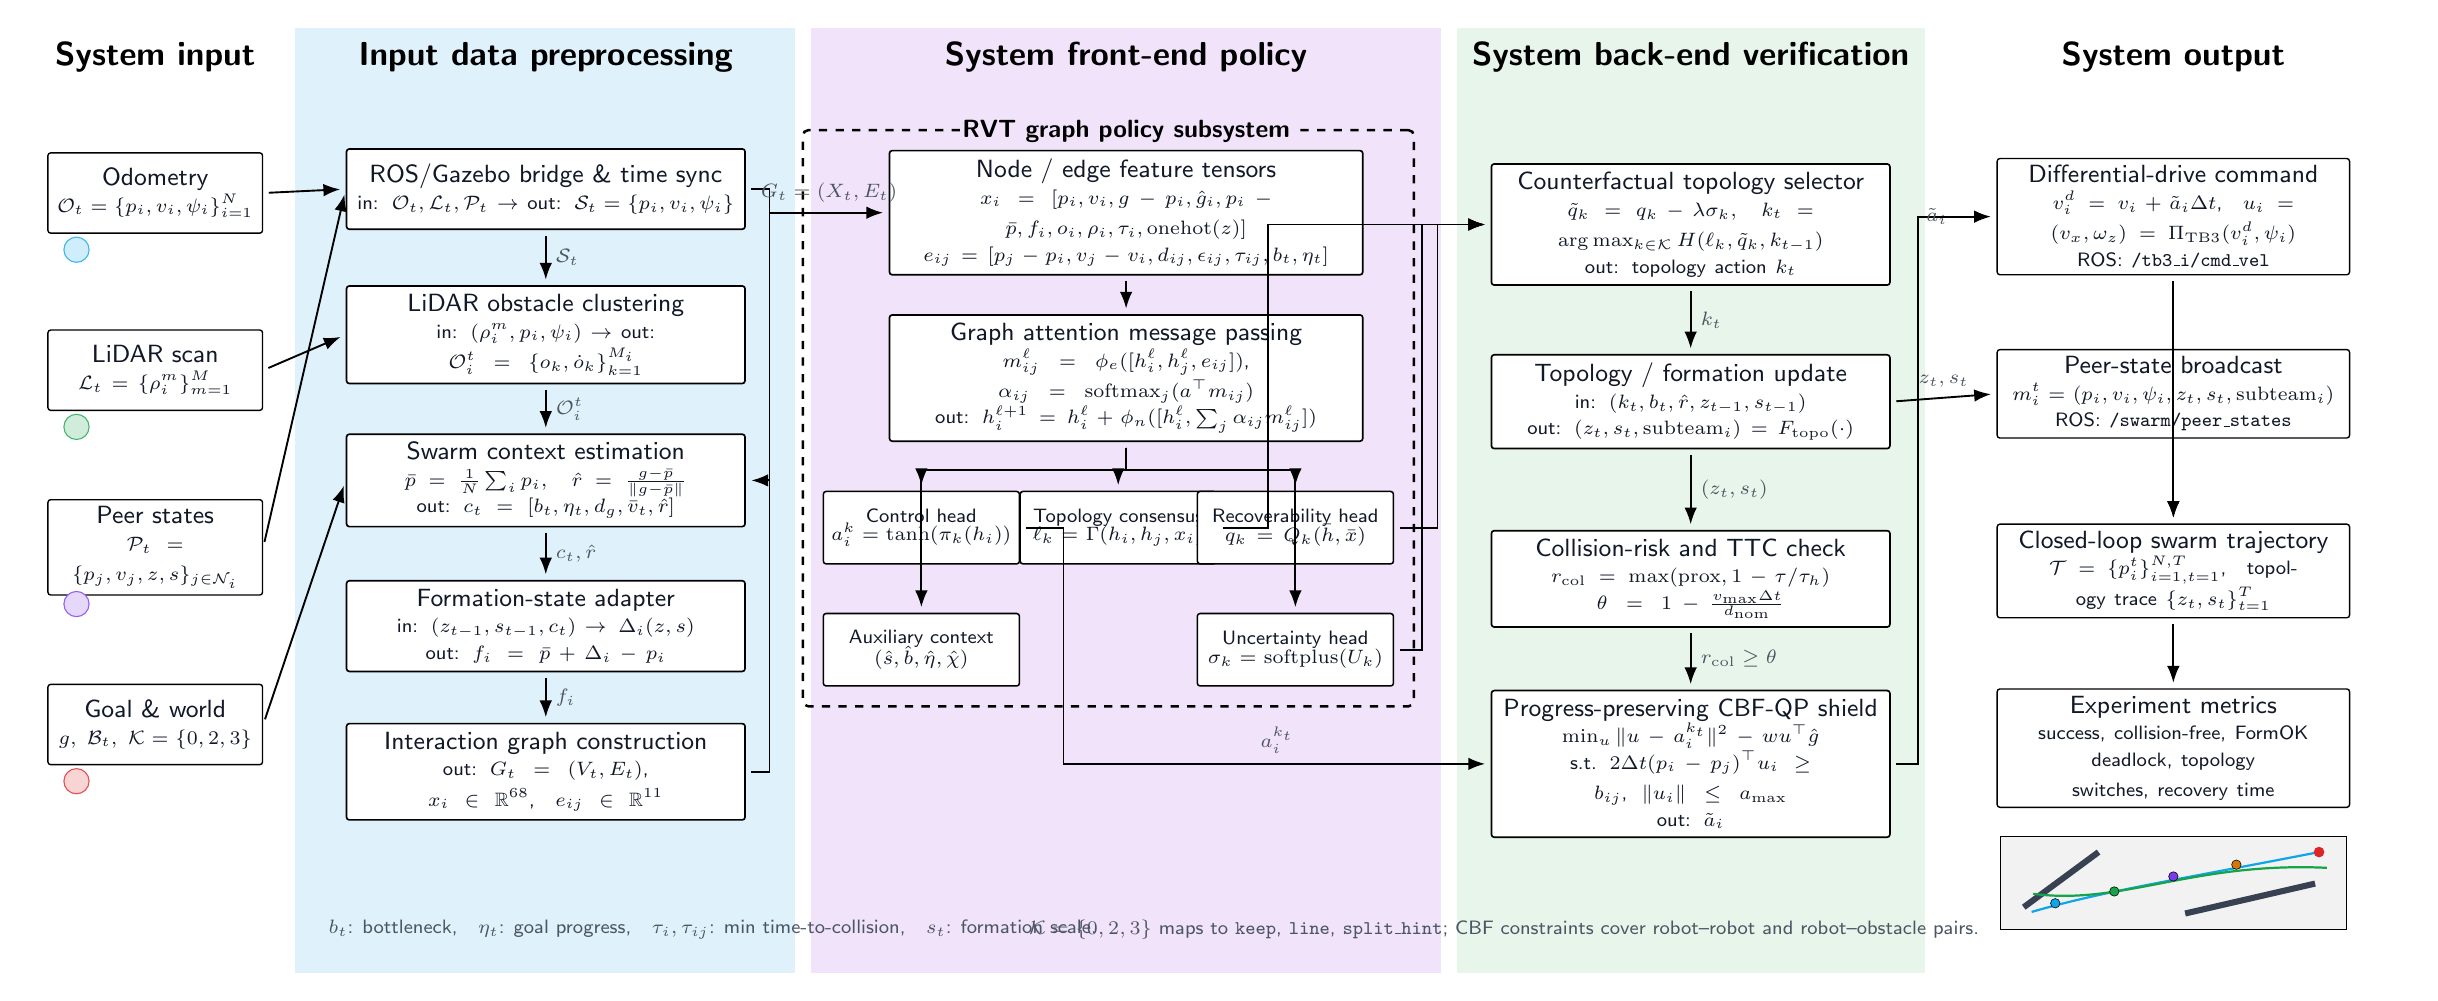
\begin{tikzpicture}[x=1cm,y=1cm]
  \def\Ytop{12.00}
  \def\Ybot{0.00}

  % Colored system regions.
  \fill[white]  (0.0,\Ybot) rectangle (3.25,\Ytop);
  \fill[prebg]  (3.40,\Ybot) rectangle (9.75,\Ytop);
  \fill[frontbg](9.95,\Ybot) rectangle (17.95,\Ytop);
  \fill[backbg] (18.15,\Ybot) rectangle (24.10,\Ytop);
  \fill[white]  (24.30,\Ybot) rectangle (30.25,\Ytop);

  \node[sectiontitle] at (1.62,11.62) {System input};
  \node[sectiontitle] at (6.58,11.62) {Input data preprocessing};
  \node[sectiontitle] at (13.95,11.62) {System front-end policy};
  \node[sectiontitle] at (21.12,11.62) {System back-end verification};
  \node[sectiontitle] at (27.25,11.62) {System output};

  % Inputs.
  \node[ioitem] (odom) at (1.62,9.90)
    {Odometry\\[-0.5mm]{\scriptsize $\mathcal O_t=\{p_i,v_i,\psi_i\}_{i=1}^{N}$}};
  \node[ioitem] (scan) at (1.62,7.65)
    {LiDAR scan\\[-0.5mm]{\scriptsize $\mathcal L_t=\{\rho_i^m\}_{m=1}^{M}$}};
  \node[ioitem] (peer) at (1.62,5.40)
    {Peer states\\[-0.5mm]{\scriptsize $\mathcal P_t=\{p_j,v_j,z,s\}_{j\in\mathcal N_i}$}};
  \node[ioitem] (goal) at (1.62,3.15)
    {Goal \& world\\[-0.5mm]{\scriptsize $g,\;\mathcal B_t,\;\mathcal K=\{0,2,3\}$}};

  % Minimal icon markers.
  \draw[fill=blue!20,draw=blue!80] (0.62,9.18) circle (0.16);
  \draw[fill=green!20,draw=green!80] (0.62,6.93) circle (0.16);
  \draw[fill=violet!20,draw=violet!80] (0.62,4.68) circle (0.16);
  \draw[fill=red!20,draw=red!80] (0.62,2.43) circle (0.16);

  % Preprocessing.
  \node[block] (sync) at (6.58,9.95)
    {ROS/Gazebo bridge \& time sync\\[-0.5mm]
    {\scriptsize in: $\mathcal O_t,\mathcal L_t,\mathcal P_t$
    $\rightarrow$ out: $\mathcal S_t=\{p_i,v_i,\psi_i\}$}};
  \node[block] (cluster) at (6.58,8.10)
    {LiDAR obstacle clustering\\[-0.5mm]
    {\scriptsize in: $(\rho_i^m,p_i,\psi_i)$
    $\rightarrow$ out: $\mathcal O_i^t=\{o_k,\dot o_k\}_{k=1}^{M_i}$}};
  \node[block] (context) at (6.58,6.25)
    {Swarm context estimation\\[-0.5mm]
    {\scriptsize $\bar p=\frac1N\sum_i p_i,\quad
    \hat r=\frac{g-\bar p}{\|g-\bar p\|}$}\\[-0.5mm]
    {\scriptsize out: $c_t=[b_t,\eta_t,d_g,\bar v_t,\hat r]$}};
  \node[block] (formation) at (6.58,4.40)
    {Formation-state adapter\\[-0.5mm]
    {\scriptsize in: $(z_{t-1},s_{t-1},c_t)$
    $\rightarrow \Delta_i(z,s)$}\\[-0.5mm]
    {\scriptsize out: $f_i=\bar p+\Delta_i-p_i$}};
  \node[block] (graph) at (6.58,2.55)
    {Interaction graph construction\\[-0.5mm]
    {\scriptsize out: $G_t=(V_t,E_t)$,\quad
    $x_i\in\mathbb R^{68}$,\quad $e_{ij}\in\mathbb R^{11}$}};

  % Front-end.
  \node[frontblock] (features) at (13.95,9.65)
    {Node / edge feature tensors\\[-0.5mm]
    {\scriptsize $x_i=[p_i,v_i,g-p_i,\hat g_i,p_i-\bar p,f_i,o_i,\rho_i,\tau_i,\mathrm{onehot}(z)]$}\\[-0.5mm]
    {\scriptsize $e_{ij}=[p_j-p_i,v_j-v_i,d_{ij},\epsilon_{ij},\tau_{ij},b_t,\eta_t]$}};
  \node[frontblock] (mp) at (13.95,7.55)
    {Graph attention message passing\\[-0.5mm]
    {\scriptsize $m_{ij}^{\ell}=\phi_e([h_i^\ell,h_j^\ell,e_{ij}])$,\quad
    $\alpha_{ij}=\mathrm{softmax}_j(a^\top m_{ij})$}\\[-0.5mm]
    {\scriptsize out: $h_i^{\ell+1}=h_i^\ell+\phi_n([h_i^\ell,\sum_j\alpha_{ij}m_{ij}^{\ell}])$}};
  \node[headblock] (acthead) at (11.35,5.65)
    {Control head\\[-0.5mm]{\scriptsize $a_i^k=\tanh(\pi_k(h_i))$}};
  \node[headblock] (tophead) at (13.85,5.65)
    {Topology consensus\\[-0.5mm]{\scriptsize $\ell_k=\Gamma(h_i,h_j,x_i)$}};
  \node[headblock] (rech) at (16.10,5.65)
    {Recoverability head\\[-0.5mm]{\scriptsize $q_k=Q_k(\bar h,\bar x)$}};
  \node[headblock] (unch) at (16.10,4.10)
    {Uncertainty head\\[-0.5mm]{\scriptsize $\sigma_k=\mathrm{softplus}(U_k)$}};
  \node[headblock] (auxh) at (11.35,4.10)
    {Auxiliary context\\[-0.5mm]{\scriptsize $(\hat s,\hat b,\hat\eta,\hat\chi)$}};

  \node[dashedframe, fit=(features)(mp)(acthead)(tophead)(rech)(unch)(auxh),
        inner xsep=0.25cm, inner ysep=0.25cm] {};
  \node[font=\bfseries\small,fill=frontbg,inner sep=1pt] at (13.95,10.68) {RVT graph policy subsystem};

  % Back-end.
  \node[block] (selector) at (21.12,9.50)
    {Counterfactual topology selector\\[-0.5mm]
    {\scriptsize $\tilde q_k=q_k-\lambda\sigma_k,\quad
    k_t=\arg\max_{k\in\mathcal K}H(\ell_k,\tilde q_k,k_{t-1})$}\\[-0.5mm]
    {\scriptsize out: topology action $k_t$}};
  \node[block] (runtime) at (21.12,7.25)
    {Topology / formation update\\[-0.5mm]
    {\scriptsize in: $(k_t,b_t,\hat r,z_{t-1},s_{t-1})$}\\[-0.5mm]
    {\scriptsize out: $(z_t,s_t,\mathrm{subteam}_i)=F_{\mathrm{topo}}(\cdot)$}};
  \node[block] (risk) at (21.12,5.00)
    {Collision-risk and TTC check\\[-0.5mm]
    {\scriptsize $r_{\mathrm{col}}=\max(\mathrm{prox},1-\tau/\tau_h)$}\\[-0.5mm]
    {\scriptsize $\theta=1-\frac{v_{\max}\Delta t}{d_{\mathrm{nom}}}$}};
  \node[block] (shield) at (21.12,2.65)
    {Progress-preserving CBF-QP shield\\[-0.5mm]
    {\scriptsize $\min_u\|u-a_i^{k_t}\|^2-wu^\top\hat g$}\\[-0.5mm]
    {\scriptsize s.t. $2\Delta t(p_i-p_j)^\top u_i\ge b_{ij}$,\;
    $\|u_i\|\le a_{\max}$}\\[-0.5mm]
    {\scriptsize out: $\tilde a_i$}};

  % Outputs.
  \node[outitem] (cmd) at (27.25,9.60)
    {Differential-drive command\\[-0.5mm]
    {\scriptsize $v_i^d=v_i+\tilde a_i\Delta t$,\quad
    $u_i=(v_x,\omega_z)=\Pi_{\mathrm{TB3}}(v_i^d,\psi_i)$}\\[-0.5mm]
    {\scriptsize ROS: \texttt{/tb3\_i/cmd\_vel}}};
  \node[outitem] (peerout) at (27.25,7.35)
    {Peer-state broadcast\\[-0.5mm]
    {\scriptsize $m_i^t=(p_i,v_i,\psi_i,z_t,s_t,\mathrm{subteam}_i)$}\\[-0.5mm]
    {\scriptsize ROS: \texttt{/swarm/peer\_states}}};
  \node[outitem] (traj) at (27.25,5.10)
    {Closed-loop swarm trajectory\\[-0.5mm]
    {\scriptsize $\mathcal T=\{p_i^t\}_{i=1,t=1}^{N,T}$,\quad
    topology trace $\{z_t,s_t\}_{t=1}^{T}$}};
  \node[outitem] (metrics) at (27.25,2.85)
    {Experiment metrics\\[-0.5mm]
    {\scriptsize success, collision-free, FormOK}\\[-0.5mm]
    {\scriptsize deadlock, topology switches, recovery time}};

  % Mini output visualization.
  \begin{scope}[shift={(25.05,0.55)}]
    \draw[fill=gray!10,draw=black,line width=0.35pt] (0,0) rectangle (4.40,1.18);
    \draw[darkbox,line width=2.2pt] (0.30,0.28) -- (1.25,0.98);
    \draw[darkbox,line width=2.2pt] (2.35,0.20) -- (4.00,0.58);
    \draw[blue,line width=0.8pt] (0.40,0.22) .. controls (1.30,0.48) and (2.20,0.62) .. (4.05,0.98);
    \draw[green,line width=0.8pt] (0.42,0.45) .. controls (1.55,0.30) and (2.45,0.86) .. (4.15,0.78);
    \draw[red,fill=red] (4.05,0.98) circle (0.06);
    \foreach \x/\y/\c in {0.70/0.33/blue,1.45/0.48/green,2.20/0.67/violet,3.00/0.82/amber}
      \draw[fill=\c,draw=black,line width=0.2pt] (\x,\y) circle (0.06);
  \end{scope}

  % Arrows: inputs to preprocessing.
  \draw[arrow] (odom.east) -- (sync.west);
  \draw[arrow] (scan.east) -- (cluster.west);
  \draw[arrow] (peer.east) -- (sync.west);
  \draw[arrow] (goal.east) -- (context.west);

  % Preprocessing flow.
  \draw[arrow] (sync) -- node[formula,right] {$\mathcal S_t$} (cluster);
  \draw[arrow] (sync.east) -- ++(0.30,0) |- (context.east);
  \draw[arrow] (cluster) -- node[formula,right] {$\mathcal O_i^t$} (context);
  \draw[arrow] (context) -- node[formula,right] {$c_t,\hat r$} (formation);
  \draw[arrow] (formation) -- node[formula,right] {$f_i$} (graph);
  \draw[arrow] (graph.east) -- ++(0.30,0) |- node[formula,near end,above] {$G_t=(X_t,E_t)$} (features.west);

  % Front-end flow.
  \draw[arrow] (features) -- (mp);
  \draw[arrow] (mp.south) -- ++(0,-0.35) -| (acthead.north);
  \draw[arrow] (mp.south) -- ++(0,-0.35) -| (tophead.north);
  \draw[arrow] (mp.south) -- ++(0,-0.35) -| (rech.north);
  \draw[arrow] (mp.south) -- ++(0,-0.35) -| (unch.north);
  \draw[arrow] (mp.south) -- ++(0,-0.35) -| (auxh.north);

  % Front-end to back-end.
  \draw[arrow] (tophead.east) -- ++(0.65,0) |- (selector.west);
  \draw[arrow] (rech.east) -- ++(0.55,0) |- (selector.west);
  \draw[arrow] (unch.east) -- ++(0.35,0) |- (selector.west);
  \draw[arrow] (selector) -- node[formula,right] {$k_t$} (runtime);
  \draw[arrow] (runtime) -- node[formula,right] {$(z_t,s_t)$} (risk);
  \draw[arrow] (risk) -- node[formula,right] {$r_{\mathrm{col}}\ge\theta$} (shield);
  \draw[arrow] (acthead.east) -- ++(0.55,0) |- node[formula,near end,above] {$a_i^{k_t}$} (shield.west);

  % Output flow.
  \draw[arrow] (shield.east) -- ++(0.35,0) |- node[formula,near end,left] {$\tilde a_i$} (cmd.west);
  \draw[arrow] (runtime.east) -- node[formula,above] {$z_t,s_t$} (peerout.west);
  \draw[arrow] (cmd) -- (traj);
  \draw[arrow] (peerout) -- (traj);
  \draw[arrow] (traj) -- (metrics);

  % Legend.
  \node[font=\scriptsize,align=left,text=muted] at (8.70,0.55)
    {$b_t$: bottleneck,\quad $\eta_t$: goal progress,\quad
     $\tau_i,\tau_{ij}$: min time-to-collision,\quad $s_t$: formation scale.};
  \node[font=\scriptsize,align=left,text=muted] at (18.75,0.55)
    {$\mathcal K=\{0,2,3\}$ maps to \texttt{keep}, \texttt{line}, \texttt{split\_hint}; CBF constraints cover robot--robot and robot--obstacle pairs.};
\end{tikzpicture}
\end{document}
